\chapter{Der Detroit im aktuellen Zustand}

\section{Batterie}
Als Batterie für den Detroit sollten die modernen Lithium-Ionen-Akkumulatoren des Peugeot-Unfallfahrzeuges verwendet werden. Dabei mussten jedoch einige Anpassungen vorgenommen werden, da die Batterien zum einen nicht die selbe Spannung besassen, zum anderen beim Detroit auch zwei unabhängige Batterien verbaut waren. Dies zog umfangreiche Anpassungen mit sich, die nachfolgend erläutert werden.

\subsection{Funktion von Lithium-Ionen-Akkumulatoren} \label{kap_liion}

Lithium-Ionen-Akkumulatoren sind in der heutigen Zeit Standard. Das heisst in allen neuartigen Handys, Mobiltelefonen aber auch in Fahrzeugen werden diese verbaut und es wird immer mehr auf Blei-Akkus verzichtet. Die Technologie um die Lithium-Ionen Akkus ist jedoch im Vergleich zu Blei-Batterien sehr jung, genauer gesagt ca. 50 Jahre alt, und hinter den effizienten Akkus liegt eine aufwändige Ladetechnik. Nachfolgend wird kurz die Funktionsweise und die Lade-/Entladekurve der Lithium-Ionen-Akkus erläutert.

\paragraph{Aufbau/Grundfunktion}

Der Name Lithium-Ionen-Akkumulator kommt von den Lithiumionen die frei zwischen den beiden Elektroden wandern. Durch einen Separator sind die beiden Elektroden durch direkten Kontakt geschützt. Die positive Elektrode besteht aus Lithium-Metalloxide wie zum Beispiel LiCoO$_2$, LiNiO$_2$ oder LiMn$_2$O$_4$ und die negative aus Graphit. Wichtig ist, dass die Elektrolytlösung frei von Wasser ist, damit es nicht mit dem Lithium reagiert.
Grundsätzlich funktioniert der Akku so, dass im Ladevorgang positiv geladene Lithiumionen von der positiven zur negativen Elektrode übergehen und an der Kathode hängen bleiben. Gleichzeitig liefert der Ladestrom die Elektronen über eine von aussen angelegte Verbindung. Beim Entladevorgang funktioniert wieder das umgekehrte. Die Elektronen fliessen über den äusseren Stromkreis zur positiven Elektrode. Der Aufbau und die Grundfunktion sind in Figur \ref{fig:liion_akku} dargestellt. \cite{liion_akku_aufbau_funktion2}

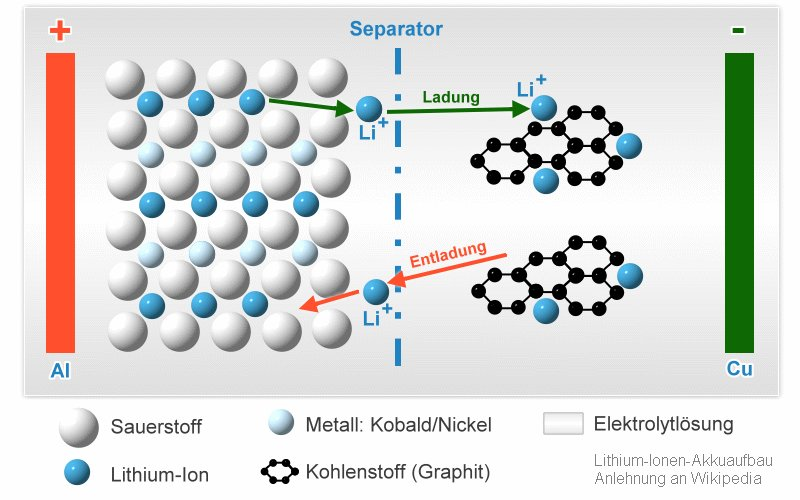
\includegraphics[width=0.75\textwidth]{images/aufbau_liion.jpg}
	\caption{Aufbau/Grundfunktion Lithium-Ionen-Akkumulator \cite{liion_akku_aufbau_funktion1}}
	\label{fig:liion_akku}
\end{figure}

\paragraph{Lade-/Entladekurve}

Die typische Ladekurve ist nachfolgend aufgeführt:

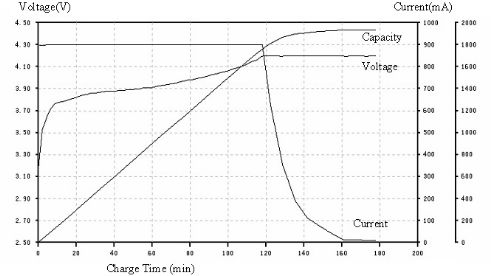
\includegraphics[width=0.75\textwidth]{images/liion_laden.jpg}
	\caption{Ladekurve Lithium-Ionen-Akkumulator \cite{liion_kurve}}
	\label{fig:liion_akku_kurve}
\end{figure}

Es ist zu sehen, dass die Batteriespannung innert kurzer Zeit stark ansteigt. Das heisst im Bild von etwa 0 bis 10 Minuten. Von 10 Minuten bis 130 Minuten wird die Steigung flacher. Von 120 Minuten bis ca. 180 Minuten bleibt die Spannung konstant, bis dann 100\% der Kapazität erreicht wird.

Leider wurden keine korrekten Kurven für Entladevorgänge gefunden. \todo{für Entladevorgänge bessere Beschreibung}

\subsection{Vergleich Blei / Lithium-Ionen} \label{kap:Vergleich_liion_pb}

Um die Unterschiede, bzw. Vor- und Nachteile von Lithium-Ionen zu Blei-Akkus besser zu verstehen, sind nachfolgend kurz einige Argumente aufgelistet:

\paragraph{Vorteil Blei}

Kurzfristige Lieferung von hohen Strömen ist für Blei-Akkumulatoren kein Problem. Auch besitzen sie ein gutes Preis-/Leistungsverhältnis und sehr zuverlässig, wenn Wartung und Pflege eingehalten werden.

\paragraph{Nachteil Blei}

Die Energiedichte ist sehr gering. Das heisst es braucht ein grosses Volumen um überhaupt ansatzweise eine gute Kapazität zu erreichen. Das Elektrolyt ist säurehaltig, womit Verätzungsgefahr besteht. Zusätzlich